\section{STRIDE Modeling}

\begin{figure}[h!]
\centering
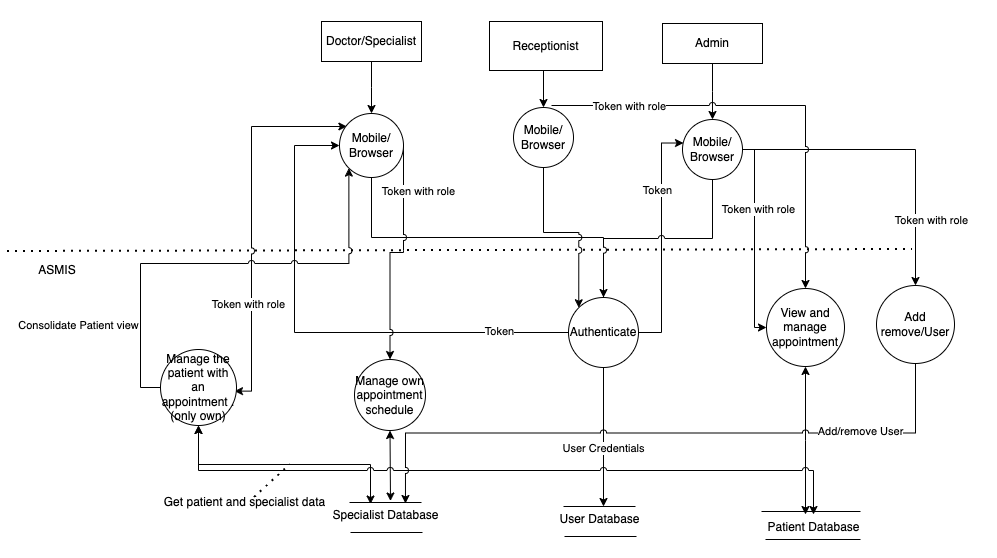
\includegraphics[width=\textwidth]{pics/dfd_staff.png}
\caption{DFD level 0 Staff for ASMIS}\label{fig:dfd_staff}
\end{figure}

\begin{figure}[h!]
\centering
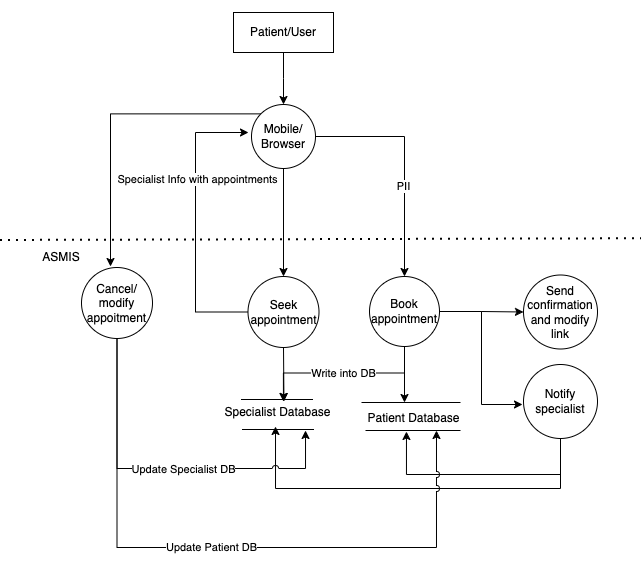
\includegraphics[width=12cm, height=11cm]{pics/dfd_user.png}
\caption{DFD level 0 User for ASMIS}\label{fig:dfd_user}
\end{figure}

\subsection{Overview}
STRIDE is one of the most mature threat analysis modeling methods. Microsoft has adopted this method since 2002, where STRIDE stands for a mnemonic, Spoofing, Tampering, Repudiation, Information disclosure, Denial of Service, and Elevation of privilege. It is also easier to discover and brainstorm possible threats using these points. Its simplicity and ability to find threats using dataflow diagrams made it a promising candidate for this report.\newline\newline
Figures \ref{fig:dfd_staff} and \ref{fig:dfd_user} depict the Level 0 dataflow diagram in respect to the different actors and how the system acts between the trusted boundaries. Additionally, from the DFD, we can identify the events and boundaries of the ASMIS system that would provide a concrete platform to perform STRIDE modeling \citep[p.~1]{shevchenko2018threat}.

\subsection{Spoofing}
\begin{enumerate}    
  \item Take over Staff account 
  \item DNS spoofing to redirect users to a fake site
  \item Ip spoofing
  \item Attacker can pose as an unauthenticated user to make appointments unavailable.
  \item Replay attacks
  \item Man-in-the-middle-attack
\end{enumerate}
\subsubsection{Mitigations}
\begin{enumerate}
    \item Having strict Multifactor authentication rules for the staff. Using only app-based or hardware key-based MFA solutions.
    \item Keeping the validity of the access tokens short-lived.
    \item Use only one-time usable refresh tokens and blacklist all tokens if the refresh token is used more than once.
    \item Use encrypted protocols, i.e, HTTPS everywhere to communicate.
    \item Use DNSSec to prevent cache poisoning.
\end{enumerate}

\subsection{Tampering}
\begin{enumerate}    
  \item Tampering roles in a token of an authorized user
  \item Modify mobile app or browser app code.
   \item Redirect data flow to an attacker's machine.
   \item Cross-Site Request Forgery.
   \item Modify a patient's appointments without authority.
\end{enumerate}
\subsubsection{Mitigations}
\begin{enumerate}
    \item Digital signatures using a safely stored private key on the tokens should be carried out.
    \item Using checksums to test the recognized codes.
    \item Sending OTP to patient's verified phone, before being able to modify appointments.
    \item Using CSRF token to verify, if the 
\end{enumerate}

\subsection{Redupation}
\begin{enumerate}    
  \item Claims to be some other user/staff
  \item Modify mobile app or browser app code
  \item User claims not to have set up or canceled an appointment.
\end{enumerate}

\subsubsection{Mitigations}
\begin{enumerate}
    \item 
\end{enumerate}

\subsection{Information Disclousre}
\begin{enumerate}
    \item Vital system errors in error logs
    \item SQL injection to get data from the database
    \item private keys stored securely in local storage of browser/mobile
    \item Get information for analyzing the traffic
    \item Benefiting from loose ACL
\end{enumerate}

\subsection{Denial of Service}
\begin{enumerate}
    \item Attempt too many logins for staff
    \item Use bots to carry out Syn flood attacks on the application.
    \item Bots pose as users and book all available appointments.
\end{enumerate}

\subsection{Elevation of Privilege}
\begin{enumerate}
    \item Admin Privileges to all the staff
    \item Other users allowed to add roles to itself
    \item A super user for the application, which could access all the resources.
\end{enumerate}